\documentclass{article}

\usepackage{inputenc}
\usepackage{fontenc}
\usepackage{array}
\usepackage{graphicx}
\usepackage{hyperref}
\usepackage[ngerman]{babel}
\usepackage{tabularx}
\usepackage{biblatex}
\usepackage{csquotes}
\usepackage{titling}
\usepackage{parskip}
\usepackage{placeins}
\usepackage{float}
\usepackage{geometry}

\addbibresource{.bib}

\geometry{a4paper, top=25mm, left=25mm, right=25mm, bottom=25mm}

\tolerance=1000

\title{\Huge{Gesammeltes Wissen} \\ \Large{in der Ausbildung zum Fachinformatiker Anwendungsentwicklung in Köln 2023 bis 2026}}
\author{Leon Ziegenhagen}
\date{Stand: \today}

\setcounter{tocdepth}{2}
\setcounter{secnumdepth}{0}

\AddToHook{cmd/section/before}{\clearpage}

\begin{document}

\maketitle
\clearpage

\tableofcontents
\clearpage

\section{Einleitung}

Dieses Dokument dient als Sammlung und Dokumentation des erlernten Wissens im Rahmen der Ausbildung zum Fachinformatiker in der Fachrichtung Anwendungsentwicklung. Es ist ein umfassender Überblick über die Ausbildungsinhalte, die im Verlauf der dreijährigen Berufsausbildung bei der AXA AG und insbesondere am Georg-Simon-Ohm Berufskolleg in Köln 2023 bis 2026 vermittelt wurden. Ziel dieses Dokumentes ist es, die wesentlichen Lerninhalte zu strukturieren und so eine verständliche Übersicht über die verschiedenen Fachthemen zu bieten, die während der Ausbildung behandelt wurden.

Dieses Dokument nennt hauptsächlich theoretisches Wissen, welches in der Berufsschule vermittelt wurde und oder welches von der IHK verlangt und geprüft wird.

Für die Ausbildung ist das duale System vorgeschrieben. Diese hat sich in Deutschland ganz besonders erfolgreich erwiesen, da es den Auszubildenden ermöglicht, ihre theoretischen Kenntnisse in der Berufsschule mit praktischen Erfahrungen im Ausbildungsbetrieb zu kombinieren. Die Struktur des dualen Systems ist dabei klar gegliedert und findet auf verschiedenen Ebenen statt:

\begin{figure}[H]
    \centering
    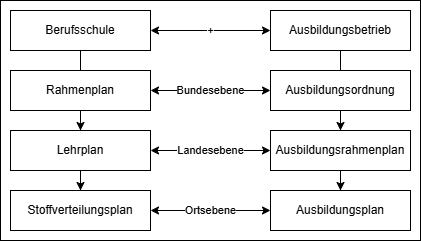
\includegraphics[width=\textwidth]{figures/dualesSystem.png}
    \caption{Duales System}
    \label{fig:dualesSystem}
\end{figure}
\FloatBarrier

Im Ausbildungsrahmenplan werden die Lernfelder wie in folgenden Kapiteln gegliedert. Darüber hinaus sieht das Land Nordrhein-Westfalen die Verknüpfung verschiedener Lernfelder in sog. Bündelungsfächer. Diese sind Gestaltung von IT-Dienstleistungen (GID), Wirtschaft- und Betriebslehre (WuB), Entwicklung vernetzter Prozesse (EvP), Cyber-Physische System (CPS), Softwaretechnologie und Datenmanagement (SuD) und IT-Grundrecht (ITG).

\begin{table}[H]
    \centering
    \begin{tabularx}{\textwidth}{|c|>{\centering\arraybackslash}X|>{\centering\arraybackslash}X|>{\centering\arraybackslash}X|>{\centering\arraybackslash}X|}
        \hline
               & GID und WuB & EvP und CPS & SuD & ITG \\
        \hline
        LF 1   & X           &             &     &     \\
        \hline
        LF 2   & X           &             &     &     \\
        \hline
        LF 3   &             & X           &     &     \\
        \hline
        LF 4   &             &             &     & X   \\
        \hline
        LF 5   &             &             & X   &     \\
        \hline
        LF 6   & X           &             &     &     \\
        \hline
        LF 7   &             & X           &     &     \\
        \hline
        LF 8   &             &             & X   &     \\
        \hline
        LF 9   &             & X           &     &     \\
        \hline
        LF 10a &             &             &     &     \\
        \hline
        LF 11a &             &             &     &     \\
        \hline
        LF 12a &             &             &     &     \\
        \hline
    \end{tabularx}
    \caption{Bündelungsfächer zu Lernfeldern}
    \label{tab:buendelfaecher}
\end{table}
\FloatBarrier

\section{Lernfeld 1: Das Unternehmen und die eigene Rolle im Betrieb beschreiben}

\begin{figure}[H]
    \centering
    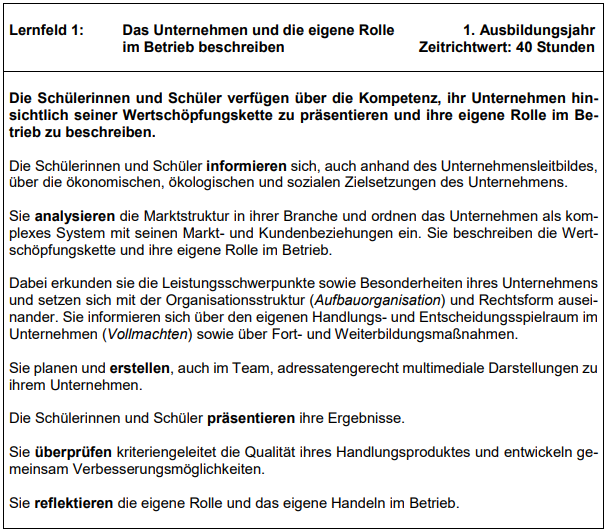
\includegraphics[width=\textwidth]{figures/lernfeld1.png}
    \caption{Lernfeld 1}
    \label{fig:lernfeld1}
\end{figure}
\FloatBarrier

\subsection{Unternehmensleitbild}
Ein Unternehmensleitbild beschreibt das Selbstverständnis und die Grundsätze eines Unternehmens. Es richtet sich an Mitarbeiter, Kunden und an die Öffentlichkeit. Es beinhaltet:

\begin{itemize}
    \item Vision / Selbstverständnis
    \item Mission / Ziel
    \item Grundsätze / Strategie
\end{itemize}

Das Leitbild verdeutlicht den Sinn und Zweck des Unternehmens und trägt zur Imagepflege bei. Ein erfolgreiches Leitbild sollte folgendes bewirken:

\begin{itemize}
    \item Motivierte und unternehmen-gebundene Mitarbeiter
    \item Grundlage für Unternehmensziele und Strategien
    \item Klare und zur Konkurrenz differenzierte Unternehmensidentität
    \item Entscheidungshilfe für Führungskräfte
    \item Hilfestellung in Konfliktsituationen
    \item Vereinfachte Personalauswahl
\end{itemize}

\subsection{Unternehmensziele}
Unternehmensziele leiten sich oft aus den im Unternehmensleitbild formulierten Grundsätzen und Visionen ab. Unternehmensziele sollten allerdings konkret und messbar ausformuliert werden. Diese Ziele lassen sich folgendermaßen kategorisieren:

\begin{itemize}
    \item Sachziele
    \item Ökonomische Ziele
    \item Ökologische Ziele
    \item Soziale Ziele
\end{itemize}

Dabei sind erwerbswirtschaftliche Unternehmen i.d.R. an Gewinnmaximierung, Rentabilität und oder hohem Marktanteil interessiert wohingegen öffentliche Unternehmen i.d.R. an Bedarfsdeckung, Kostendeckung, Verlustminimierung und oder angemessenem Gewinn interessiert sind. Der Aspekt Nachhaltigkeit ist für alle Unternehmen unter den Aspekten des Images, des Umsatzes, der Kostensenkung und der ökologisch-sozialen Verantwortung interessant.

Unternehmensziele können komplementär, konkurrierend oder neutral einander gegenüberstehen.

\textbf{Shareholder und Stakeholder}

Shareholder sind Anteilseigner bzw. Kapitalgeber. Stakeholder sind unabhängig von ihrer finanzielle Beteiligung Einflussnehmer oder Betroffene von (Teil-)Unternehmen.

\subsection{Aufbauorganisation}
Die Aufbauorganisation bestimmt welche Aufgaben von welchen Personen übernommen werden. Sie grenzt sich von der Ablauforganisation ab, welche den Ablauf von Leistungs- und Produktionsprozessen bestimmt. Um eine Aufbauorganisation darzustellen bieten sich Leitungssysteme an, welche speziell Führungs- und Entscheidungsprozesse im Unternehmen organisieren. Die grafische Darstellung eines Leitungssystem ist z.B. das sog. Organigramm, welches zusätzlich Abteilungen oder Teams darstellen kann.

Leistungssysteme lassen sich folgendermaßen differenzieren:

\begin{table}[H]
    \centering
    \begin{tabularx}{\textwidth}{|c|X|X|X|X|}
        \hline
                   & Einliniensystem                                                                                                                                          & Stab-Liniensystem                                                                                                                 & Mehrliniensystem (Funktional)                                                                                                                                                                                                                             & Matrixsystem                                                                                                                                                                                                                                                        \\
        \hline
        Grundsatz  & Eine untergeordnete Stelle erhält jeweils nur von einer vorgesetzten Instanz Anweisungen. Die Linie bildet gleichzeitig den kommunikativen Dienstweg ab. & Ein um Stäbe erweitertes Einliniensystem. Die Stäbe haben keine Weisungsbefugnis sondern bereiten Entscheidungen vor und beraten. & Spezialisten sind für definierte Funktionen zuständig und unmittelbar fachlich weisungsbefugt. Anforderungen bzw. Anweisungen können von verschiedenen Vorgesetzten kommen und Instanzen auf gleicher Ebene können unmittelbar miteinander kommunizieren. & Es existieren zwei weitestgehend unabhängige Hierarchien o. Dimensionen. Z.B. können Funktionen und Objekte oder Projekte sein. An Kreuzungspunkten befinden sich fachliche Spezialisten, welche Anforderungen von überall bekommen können, aber meist autark sind. \\
        \hline
        Schema     & siehe Abb. \ref{fig:einliniensystem}                                                                                                                     & siehe Abb. \ref{fig:stabliniensystem}                                                                                             & siehe Abb. \ref{fig:mehrliniensystem}                                                                                                                                                                                                                     & siehe Abb. \ref{fig:matrixsystem}                                                                                                                                                                                                                                   \\
        \hline
        Eigenarten & Streng hierarchisches Denken und große Macht bei Leitungskräften.                                                                                        & Trennung von Entscheidungs- und Fachkompetenz.                                                                                    & Spezialisierung der Instanzen und verkürzte Delegations- und Informationswege.                                                                                                                                                                            & Autarke und schnell agierende Instanzen.                                                                                                                                                                                                                            \\
        \hline
        Vorteile   & klare Zuständigkeiten, einfach, Konflikte wg. widersprüchlichen Anweisungen unwahrscheinlich                                                             & Entlastung der Führungskräfte, Trennung und Konzentration Entscheidungs- und Fachkompetenzen                                      & höhere Flexibilität, schnellere Entscheidungsfindung, Entlastung durch Spezialisierung der Führungskräfte                                                                                                                                                 & optimierte Ressourcennutzung, Flexibilität und Dynamik, Förderung interdisziplinärer Zusammenarbeit                                                                                                                                                                 \\
        \hline
        Nachteile  & hohe Last bei Führungskräften, geringe Flexibilität, lange Kommunikationswege                                                                            & mögliche unklare Verantwortungen, Konfliktmöglichkeit zwischen Führungskraft und Stab                                             & hohes Konfliktpotential zwischen Führungskräften, unklare Verantwortlichkeiten, Komplexität                                                                                                                                                               & Konfliktpotential zwischen Führungskräften, Komplexität insbesondere der Kommunikation und Koordination, Hoher Abstimmungsaufwand für die Gesamtunternehmensplanung                                                                                                 \\
        \hline
    \end{tabularx}
    \caption{Leitungssysteme}
    \label{tab:leitungssysteme}
\end{table}


\begin{figure}[H]
    \centering
    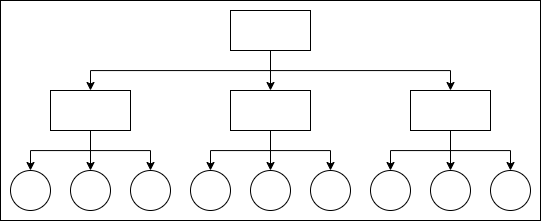
\includegraphics[width=\textwidth]{figures/einliniensystem.png}
    \caption{Einliniensystem}
    \label{fig:einliniensystem}
\end{figure}
\FloatBarrier

\begin{figure}[H]
    \centering
    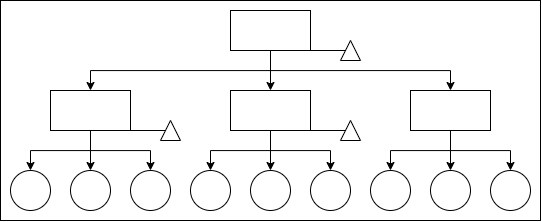
\includegraphics[width=\textwidth]{figures/stabliniensystem.png}
    \caption{Stab-Liniensystem}
    \label{fig:stabliniensystem}
\end{figure}
\FloatBarrier

\begin{figure}[H]
    \centering
    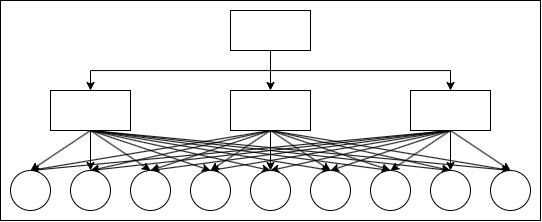
\includegraphics[width=\textwidth]{figures/mehrliniensystem.png}
    \caption{Mehrliniensystem}
    \label{fig:mehrliniensystem}
\end{figure}
\FloatBarrier

\begin{figure}[H]
    \centering
    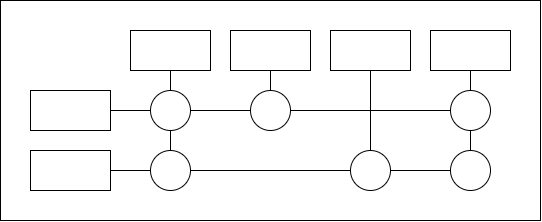
\includegraphics[width=\textwidth]{figures/matrixsystem.png}
    \caption{Matrixsystem}
    \label{fig:matrixsystem}
\end{figure}
\FloatBarrier

\subsection{Rechtsformen}

Rechtsformen beziehen sich auf Unternehmen. Unternehmen sind dabei von Betrieben und Firmen folgendermaßen abzugrenzen. Unternehmen sind rechtlich selbstständige organisatorische Einheiten der Volkswirtschaft. Betriebe sind technisch-soziale Einheiten und Unternehmen unterzuordnen. Betriebe beschreiben oft örtliche Einheiten eines Unternehmens. Firmen sind im Handelsregister eingetragene Namen eines Unternehmens. Sie bestehen aus Firmenkern (eigentlicher Name) und Firmenzusatz (Rechtsform).

Der Firmenkern kann sich von Namen (Personenfirmenkern), von Produkten oder Dienstleistungen (Sachfirmenkern), aus einer Mischform (Mischfirmenkern) ableiten oder frei erfunden werden (Fantasie-Firmenkern).

\textbf{Einzelunternehmen}

Der einzelne Unternehmer hat alleiniges Bestimmungsrecht. Er bringt das gesamte notwendige Kapital auf und erhält den kompletten Gewinn. Er trägt das alleinige Risiko und haftet mit seinem gesamten Betriebs- und Privatvermögen. Es ist die häufigste Rechtsform in Deutschland.

\textbf{Personengesellschaften}

Personengesellschaften werden von mindesten zwei i.d.R. natürlichen Personen gegründet. Zu Personengesellschaften gehören u.a. die Gesellschaft bürgerlichen Rechts (GbR), die offene Handelsgesellschaft (OHG) und die Kommanditgesellschaft (KG). Gesellschafter haften für Gesellschaftsschulden persönlich. Gesellschafter sind Inhaber und meist auch Geschäftsführer.

\textbf{Kapitalgesellschaften}

Kapitalgesellschaften sind z.B. die Gesellschaft mit beschränkter Haftung (GmbH) und die Aktiengesellschaft (AG). Die Haftung ist auf Gesellschaftseinlagen beschränkt. Für die Gründung ist ein Mindestkapital notwendig. Kapitalgesellschaften sind juristische Personen und können von beliebigen Personen geführt werden.

\begin{table}[H]
    \centering
    \begin{tabularx}{\textwidth}{|>{\centering\arraybackslash}X|>{\centering\arraybackslash}X|>{\centering\arraybackslash}X|>{\centering\arraybackslash}X|>{\centering\arraybackslash}X|>{\centering\arraybackslash}X|}
        \hline
                                      & Mindest\-Gründerzahl              & Haftung                                                                                                      & Mindest\-kapital & Geschäfts\-führung                                                        & Gewinn\-verteilung                                                                                                                                      \\
        \hline
        Kleingewerbe                  & 1                                 & unbeschränkt inkl. Privatvermögen                                                                            & -                & Kleingewerbe\-treibende                                                   & Voller Gewinn an den Kleingewerbetreibenden                                                                                                             \\
        \hline
        Eingetragener Kaufmann (E.K.) & 1                                 & unbeschränkt inkl. Privatvermögen                                                                            & -                & Eingetragener Kaufmann                                                    & Voller Gewinn an den Eingetragenen Kaufmann                                                                                                             \\
        \hline
        GbR                           & 2                                 & unbeschränkt inkl. Privatvermögen                                                                            & -                & alle Gesellschafter, sofern im Gesellschaftsvertrag nicht anders geregelt & zu gleichen Teilen auf alle Gesellschafter, sofern im Gesellschaftsvertrag nicht anders geregelt                                                        \\
        \hline
        OHG                           & 2                                 & unbeschränkt inkl. Privatvermögen                                                                            & -                & alle Gesellschafter, sofern im Gesellschaftsvertrag nicht anders geregelt & min. 4\% der Einlagen eines Gesellschafters und danach zu gleichen Teilen auf alle Gesellschafter, sofern im Gesellschaftsvertrag nicht anders geregelt \\
        \hline
        KG                            & 1 Komplementär und 1 Kommanditist & Betriebsvermögen, dann Einlagen der Kommanditisten und zuletzt der Komplementär inkl. seines Privatvermögens & -                & Alle Komplementäre                                                        & min. 4\% der Einlagen eines Gesellschafters und danach oder anstelle davon durch vertragliche Regelungen                                                \\
        \hline
        GmbH                          & 1                                 & beschränkt auf das Gesellschaftsvermögen                                                                     & 25.000€          & Angestellter Geschäftsführer                                              & Gewinnanteil entsprechend des Kapitalanteils, sofern vertraglich nicht anders geregelt                                                                  \\
        \hline
        AG                            & 1                                 & beschränkt auf das Gesellschaftsvermögen                                                                     & 50.000€          & Vorstand                                                                  & Gewinnanteil entsprechend des Aktienanteil oder vertraglich geregelt z.B. mit Dividenden                                                                \\
        \hline
    \end{tabularx}
    \caption{Rechtsformen}
    \label{tab:rechtsformen}
\end{table}

Es gibt außerdem Mischformen wie die GmbH \& Co. KG, bei welcher eine KG von u.a. einer GmbH gegründet wird.

\textbf{Handelsregister}

Das Handelsregister verzeichnet Kaufleute und Firmen. Abteilung A registriert Einzelunternehmen und Personengesellschaften. Abteilung B registriert Kapitalgesellschaften.

\subsection{Vollmachten und Prokura}

Prokura ist eine Vertretungsmacht zur Geschäftsführung deren Umfang gesetzlich geregelt ist. Handlungsvollmachten begrenzen sich dagegen auf bestimmte Geschäfte.

Handlungsvollmacht ist dabei ein Oberbegriff für Generalhandlungsvollmachten und allgemeine Vollmachten, welche zum Führen des täglichen Geschäftes ermächtigen, Artvollmachten, welche sich auf einen finanziellen Rahmen oder auf einen bestimmten Handlungsbereich beschränken und Sondervollmachten, welche einmalig für explizite Geschäfte erteilt werden.

\subsection{Eigene Rolle im Betrieb}

Die eigene Rolle im Betrieb ist vorwiegend durch Rechte und Pflichten in der Ausbildung geprägt. Vor allem herrschen hier die Grundsätze des Individualrechts:

\subsubsection{Berufsbildungsgesetz (BBiG)}

Die Berufsbildung wird in Betrieben und in Berufsschulen kooperativ durchgeführt (§2 Abs. 1 und 2 BBiG).

Die Form und geforderte Inhalte einer Ausbildungsordnung ist definiert (§5 BBiG). Die Ausbildungsordnung für Fachinformatiker ist weiter unten unter FIAusbV beschrieben.

Es muss ein Ausbildungsvertrag geschlossen werden (§10 BBiG). Dieser muss folgendes beinhalten (§11 BBiG):

\begin{itemize}
    \item Name und Anschrift der Vertragsparteien
    \item Art, sachliche und zeitliche Gliederung und Ziel der Ausbildung
    \item Beginn und Dauer
    \item Ausbildungsstätte und Ausbildungsnahmen außerhalb
    \item tägliche Arbeitszeit
    \item Probezeit
    \item Vergütung
    \item Umgang mit Überstunden
    \item Urlaub
    \item Voraussetzungen für Kündigung
    \item Form des Ausbildungsnachweises
\end{itemize}

Folgende Vereinbarung sind in einer Ausbildung nichtig (§12 BBiG):

\begin{itemize}
    \item Verpflichtung zur Übernahme (außer 6 Monate vor Ausbildungsende)
    \item Verpflichtung zur Entschädigungszahlung für die Ausbildung
    \item Vertragsstrafen
    \item Ausschluss oder Beschränkung von Schadensersatzansprüchen inkl. der Festsetzung von Pauschalen bei Schadensersatz
\end{itemize}

Pflichten des Auszubildenden sind u.a. (§13 BBiG):

\begin{itemize}
    \item sorgfältig Aufgaben auszuführen
    \item Ausbildungsmaßnahmen wahrzunehmen, für welche Sie freigestellt werden
    \item Weisungen befolgen
    \item Ausbildungsstättenordnung beachten
    \item Werkzeug, Maschinen und sonstiges pfleglich behandeln
    \item Schweigepflicht über Betriebsgeheimnisse
    \item schriftlichen oder elektronischen Ausbildungsnachweis führen
\end{itemize}

Pflichten des Ausbildenden sind u.a. (§14 BBiG):

\begin{itemize}
    \item nach bestem Gewissen für den Beruf auszubilden
    \item selbst auszubilden oder ausdrücklich einen Ausbilder beauftragen
    \item Ausbildungsmittel kostenlos zur Verfügung stellen
    \item Auszubildende zum Besuch der Berufsschule anzuhalten
    \item Charakter des Auszubildenden fördern und körperliche Gefahren vermeiden
    \item Auszubildende zum Führen des Ausbildungsnachweises anzuhalten und diesen regelmäßig durchzusehen
    \item nur Aufgaben stellen, welche dem Ausbildungszweck dienen und den körperlichen Kräften des Auszubildenden angemessen sind
\end{itemize}

Auszubildende sind für die Berufsschule und Prüfungen freizustellen (§15 Abs. 1 und 2 BBiG). Für volljährige Auszubildende gilt:

\begin{table}[H]
    \centering
    \begin{tabularx}{\textwidth}{|>{\centering\arraybackslash}X|>{\centering\arraybackslash}X|}
        \hline
        Situation und Freistellung                                                                   & Anrechnung der Arbeitszeit                                                                          \\
        \hline
        Berufsschulunterricht                                                                        & Unterrichts- und Pausenzeit und notwendige Wegzeiten zwischen Berufsschule und Ausbildungsstätte    \\
        \hline
        ein Berufsschultag in der Woche mit mehr als 5 Unterrichtsstunden á 45 Min                   & durchschnittliche tägliche Arbeitszeit                                                              \\
        \hline
        Berufsschulwochen mit einem planmäßigen Blockunterricht von mindestens 25 Stunden an 5 Tagen & durchschnittliche wöchentliche Arbeitszeit                                                          \\
        \hline
        Prüfungen und Ausbildungsmaßnahmen                                                           & Zeit der Teilnahme inkl. Pausen und notwendig Wegzeiten zwischen Teilnahmeort und Ausbildungsstätte \\
        \hline
        Arbeitstag vor der AP 2                                                                      & durchschnittliche tägliche Arbeitszeit                                                              \\
        \hline
    \end{tabularx}
    \caption{Freistellung, Anrechnung}
    \label{tab:freistellung}
\end{table}

Der Ausbildende hat bei Beendigung ein Arbeitszeugnis auszustellen (§16 BBiG).

Auszubildende haben ein Anrecht auf eine Mindestvergütung mit jedem Lehrjahr steigend (§17 BBiG).

Die Probezeit darf zwischen einem und vier Monaten dauern (§20 BBiG).

Die Ausbildung endet mit Ablauf der Ausbildungsdauer oder bei bestehen der Abschlussprüfung mit Bekanntgabe der Ergebnisse (§21 Abs. 1 und 2 BBiG). Der Auszubildende kann bei nicht bestehen Verlangen das Ausbildungsverhältnis bis zur nächstmöglichen Prüfungswiederholung zu verlängern, maximal aber ein Jahr (§21 Abs. 3 BBiG).

Während der Probezeit kann jederzeit und ohne Frist gekündigt werden (§22 Abs. 1 BBiG). Nach der Probezeit darf nur aus einem wichtigen Grund und ohne Frist gekündigt werden oder vom Auszubildenden mit einer Frist von vier Wochen, wenn Sie die Ausbildung aufgeben oder eine andere Berufstätigkeit ausüben wollen (§22 Abs. 2 BBiG). Kündigungen müssen schriftlich sein und außerhalb der Probezeit den Kündigungsgrund beinhalten (§22 Abs. 3 BBiG). Eine Kündigung aus wichtigem Grund ist unwirksam, wenn dieser dem Kündigungsberechtigten länger als zwei Woche bekannt ist, außer es ist ein Güteverfahren eingeleitet, welches die Frist hemmt (22 Abs. 4 BBiG).

Werden Auszubildende nach Abschluss der Ausbildung beschäftigt ohne ausdrückliche Vereinbarung, so liegt automatisch ein Arbeitsverhältnis auf unbestimmte Zeit vor (§24 BBiG).

Die Abschlussprüfung kann bis zu zweimal wiederholt werden und ist für Auszubildende gebührenfrei. Es muss ein Zeugnis ausgestellt werden (§37 BBiG).

\textbf{Fachinformatikerausbildungsverordnung (FIAusbV)}

Die Ausbildung dauert 3 Jahre (§2 FIAusbV).

Gliederung in die Fachrichtungen Anwendungsentwicklung, Systemintegration, Daten- und Prozessanalyse und Digitale Vernetzung (§4 Abs. 1 Satz 2 FIAusbV).

Regelungen zur Abschlussprüfung finden sich in den §§ 7 bis 41 FIAusbV.

\textbf{BUrlG}

U.a. als volljähriger Auszubildender hat man einen Anspruch auf bezahlten Urlaub von mindestens 24 Werktagen pro vollem Jahr (§§ 1 bis 3 BUrlG).

\textbf{ArbSchG}

Der Arbeitgeber hat Gefahren für den Arbeitnehmer bestmöglich zu vermeiden oder gering zu halten, in dem er Maßnahmen des Arbeitsschutzes trifft und generell eine Verbesserung von Sicherheit und Gesundheitsschutz anstrebt. Der Arbeitgeber hat den Arbeitnehmer zu unterweisen und der Arbeitnehmer hat sich möglichst an die Unterweisungen und Weisungen für seinen Schutz zu halten.

\textbf{ArbZG}

Die werktägliche Arbeitszeit ist max. acht Stunden. Sie kann auf zehn Stunden verlängert werden, wenn die durchschnittliche Arbeitszeit innerhalb von 24 Wochen acht Stunden werktäglich nicht überschreitet (§3 ArbZG).

Ab einer Arbeitszeit von sechs Stunden bis zu neun Stunden sind voraus feststehende Ruhepausen von insgesamt mindestens 30 Min. und ab einer Arbeitszeit ab neun Stunden Ruhepausen von insgesamt mindestens 45 Min. einzulegen. Eine Ruhepause muss min. 15 Minuten betragen. Es darf nicht länger als sechs Stunden ohne Ruhepause gearbeitet werden (§4 ArbZG).

Zwischen den Arbeitszeiten muss eine Ruhezeit von mindestens elf Stunden liegen (§5 Abs. 1 ArbZG).

Es gilt ein generelles Beschäftigungsverbot an Sonn- und Feiertagen (§9 Abs. 1 ArbZG).

Es existieren definierte Ausnahmen und abweichende Regelungen.

\textbf{MuSchG}

\textbf{JArbSchG}

\textbf{BEEG}

\textbf{SGB IX}

\textbf{AGG}

\textbf{Sonstige}

Es sind u.a. auch das Kündigungsschutzgesetz (KSchG) und Arbeitsstättenverordnung (ArbStättV) zu beachten.

\section{Lernfeld 2: Arbeitsplätze nach Kundenwunsch ausstatten}

\begin{figure}
    [H]
    \centering
    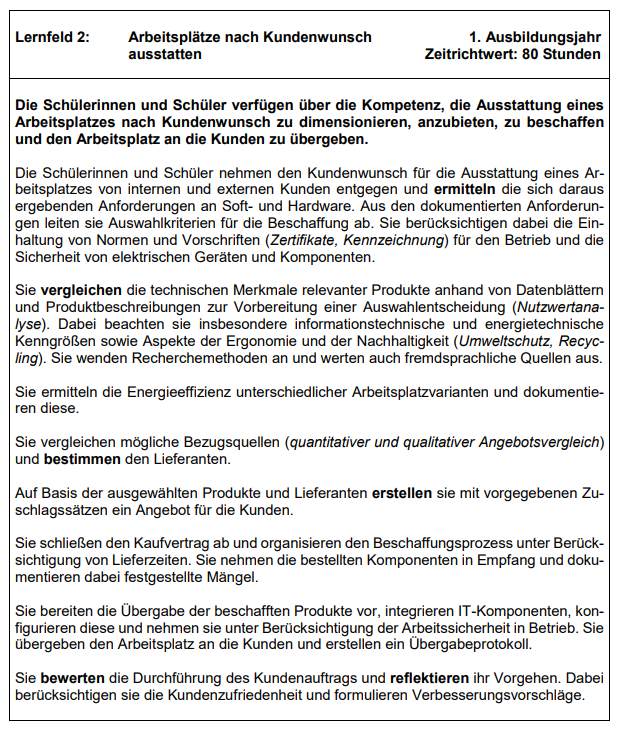
\includegraphics[width=\textwidth]{figures/lernfeld2.png}
    \caption{Lernfeld 2}
    \label{fig:lernfeld2}
\end{figure}

\subsection{Nutzwertanalyse}
Die Nutzwertanalyse (NWA) ist eine Methode des qualitativen (Angebots-)Vergleich, indem unterschiedlich bestimmte Teilnutzen zu einem Gesamtnutzen addiert werden, welcher gegen Alternativen verglichen werden kann.

\textbf{Vorgehensweise}

\begin{enumerate}
    \item Festlegen der Bewertungskriterien / Teilnutzenaspekten
    \item Festlegen der Gewichtungsfaktoren / Anteile der einzelnen Bewertungskriterien
    \item Aufstellen einer Punkteskala (z.B. Schulnoten, 0-10, 0-100)
    \item Bewertung der Entscheidungsalternativen anhand der Skala
    \item Ermitteln der gewichteten Punktwerte als Produkt aus Bewertung und Gewichtungsfaktor
    \item Summieren der gewichteten Punktwerte
    \item Interpretation der Ergebnisse
\end{enumerate}

\textbf{Beispiel}

\begin{table}[H]
    \centering
    \begin{tabularx}{\textwidth}{|>{\arraybackslash}X|c|>{\centering\arraybackslash}X|>{\centering\arraybackslash}X|>{\centering\arraybackslash}X|>{\centering\arraybackslash}X|>{\centering\arraybackslash}X|>{\centering\arraybackslash}X|}
        \hline
                    &       & \multicolumn{2}{c|}{Unternehmen 1} & \multicolumn{2}{c|}{Unternehmen 2} & \multicolumn{2}{c|}{Unternehmen 3}                                      \\
        \hline
                    & Gew.  & Punkte                             & Gew. Punkte                        & Punkte                             & Gew. Punkte & Punkte & Gew. Punkte \\
        \hline
        Grafikkarte & 20\%  & 3                                  & 60                                 & 2                                  & 40          & 4      & 80          \\
        \hline
        RAM         & 25\%  & 4                                  & 100                                & 3                                  & 75          & 4      & 100         \\
        \hline
        Monitor     & 40\%  & 2                                  & 80                                 & 1                                  & 40          & 4      & 160         \\
        \hline
        Preis       & 15\%  & 3                                  & 45                                 & 4                                  & 60          & 1      & 15          \\
        \hline
                    & 100\% &                                    & 285                                &                                    & 215         &        & 355         \\
        \hline
    \end{tabularx}
    \caption{Beispiel Nutzwertanalyse}
    \label{tab:nutzwertanalyse}
\end{table}

Die Bewertungskriterien bilden das jeweilige Teilnutzen ab. Die Größe eines Nutzens bemisst sich an denjenigen, welche das Gut nutzen, den Zweck, die Situation, der Zeitpunkt und das Gut selbst. Die Bewertungskriterien sollte untereinander nutzenunabhängig sein.

\textbf{Vorteile}

\begin{itemize}
    \item Flexibilität
    \item Schnelligkeit
    \item direkter Vergleich
    \item Eindeutigkeit
\end{itemize}

\textbf{Nachteile}

\begin{itemize}
    \item Subjektivität
    \item Manipulierbarkeit
    \item Ausschluss von Konsequenzen
    \item Niedrige Aussagekraft bei Alternativen mit sehr ähnlichen quantitativen Gesamtnutzen
\end{itemize}

\subsection{Handelskalkulation}

Die Handelskalkulation wird intern in Netto berechnet. Der Listeneinkaufspreis und Listenverkaufspreis muss für außen also ggf. in Brutto umgerechnet werden.

\textbf{Bezugskalkulation}

\begin{table}[H]
    \centering
    \begin{tabularx}{\textwidth}{c|X}
          & Listeneinkaufspreis (LEP)       \\
        \hline
        - & Lieferrabatt                    \\
        \hline
        = & Zieleinkaufspreis (ZEP)         \\
        \hline
        - & Lieferskonto                    \\
        \hline
        = & Bareinkaufspreis (BEP)          \\
        \hline
        + & Bezugskosten (z.B Lieferkosten) \\
        \hline
        = & Bezugspreis / Einstandspreis    \\
    \end{tabularx}
    \caption{Schema Bezugskalkulation}
    \label{tab:bezugskalkulation}
\end{table}

\textbf{Quantitativer Angebotsvergleich}

Mithilfe der Bezugskalkulation wird häufig ein quantitativer Angebotsvergleich durchgeführt. Dabei wird der Bezugspreis der verschiedenen Anbieter verglichen, um den günstigsten Anbieter zu ermitteln.

\textbf{Selbstkostenkalkulation im Handel}

\begin{table}[H]
    \centering
    \begin{tabularx}{\textwidth}{c|X}
          & Bezugspreis     \\
        \hline
        + & Handlungskosten \\
        \hline
        = & Selbstkosten    \\
    \end{tabularx}
    \caption{Schema Selbstkostenkalkulation}
    \label{tab:selbstkostenkalkulation}
\end{table}

Handlungskosten sind alle Kosten im Unternehmen, welche nicht direkt dem Bezug von Ware zugeordnet werden können (z.B Personalkosten, Miete, Steuer). Handlungskosten werden meist prozentual als Handlungskostenzuschlag auf den Bezugspreis aufgeschlagen. Der Handlungskostenzuschlag ist dabei das Verhältnis von Handlungskosten zu Warenaufwänden in einer Periode.

\textbf{Verkaufskalkulation}

\begin{table}
    [H]
    \centering
    \begin{tabularx}{\textwidth}{c|X}
          & Selbstkosten              \\
        \hline
        + & Gewinn                    \\
        \hline
        = & Barverkaufspreis (BVP)    \\
        \hline
        + & Kundenskonto              \\
        \hline
        = & Zielverkaufspreis (ZVP)   \\
        \hline
        + & Kundenrabatt              \\
        \hline
        = & Listenverkaufspreis (LVP) \\
    \end{tabularx}
    \caption{Schema Verkaufskalkulation}
    \label{tab:verkaufskalkulation}
\end{table}

Achtung! Der Kundenskonto bezieht sich auf den Zielverkaufspreis und nicht den Barverkaufspreis. Der Kundenrabatt bezieht sich auf den Listenverkaufspreis und nicht den Zielverkaufspreis.

Es gilt:

$ZVP = BVP + \frac{BVP * Kundenskonto}{100\% - Kundenskonto}$

und

$LVP = ZVP + \frac{ZVP * Kundenrabatt}{100\% - Kundenrabatt}$

\textbf{Vollständige Handelskalkulation Vorwärts}

Die Vorwärtskalkulation eignet sich für Märkte mit freier Preisgestaltung.

\begin{table}
    [H]
    \centering
    \begin{tabularx}{\textwidth}{c|X}
          & Listeneinkaufspreis (LEP) \\
        \hline
        - & Lieferrabatt              \\
        \hline
        = & Zieleinkaufspreis (ZEP)   \\
        \hline
        - & Lieferskonto              \\
        \hline
        = & Bareinkaufspreis (BEP)    \\
        \hline
        + & Bezugskosten              \\
        \hline
        = & Bezugspreis               \\
        \hline
        + & Handlungskosten           \\
        \hline
        = & Selbstkosten              \\
        \hline
        + & Gewinn                    \\
        \hline
        = & Barverkaufspreis (BVP)    \\
        \hline
        + & Kundenskonto              \\
        \hline
        = & Zielverkaufspreis (ZVP)   \\
        \hline
        + & Kundenrabatt              \\
        \hline
        = & Listenverkaufspreis (LVP) \\
    \end{tabularx}
    \caption{Schema Vorwärtskalkulation}
    \label{tab:vorwaertskalkulation}
\end{table}

Siehe Verkaufskalkulation für die Berechnung von ZVP und LVP.

\textbf{Rückwärtskalkulation}

Die Rückwärtskalkulation eignet sich für Märkte mit vorgegebenen Verkaufspreisen.

Das Schema der Rückwärtskalkulation ist gleich dem Schema der Vorwärtskalkulation. Allerdings ist letztere Umzudrehen, Vorzeichen werden invertiert und die besondere Berechnung vo ZVP und LVP wie in der Verkaufskalkulation wird stattdessen auf die Berechnung des ZEP und LEP angewendet.

\textbf{Differenzkalkulation}

Die Differenzkalkulation berechnet den Gewinn bei festem oder marktüblichen Listeneinkaufspreis und Listenverkaufspreis als Differenz von Selbstkosten und Barverkaufspreis. Es wird ein beliebiges Schema der Handelskalkulation verwendet und aus beiden Richtung bis zu Selbstkosten und Barverkaufspreis berechnet.

\end{document}